\begin{frame}{Traditional Numerical Methods in Geophysics}
  \begin{columns}[T,onlytextwidth]
    \begin{column}{0.48\textwidth}
      \begin{figure}
	\centering % This ensures the image is centered in the column
      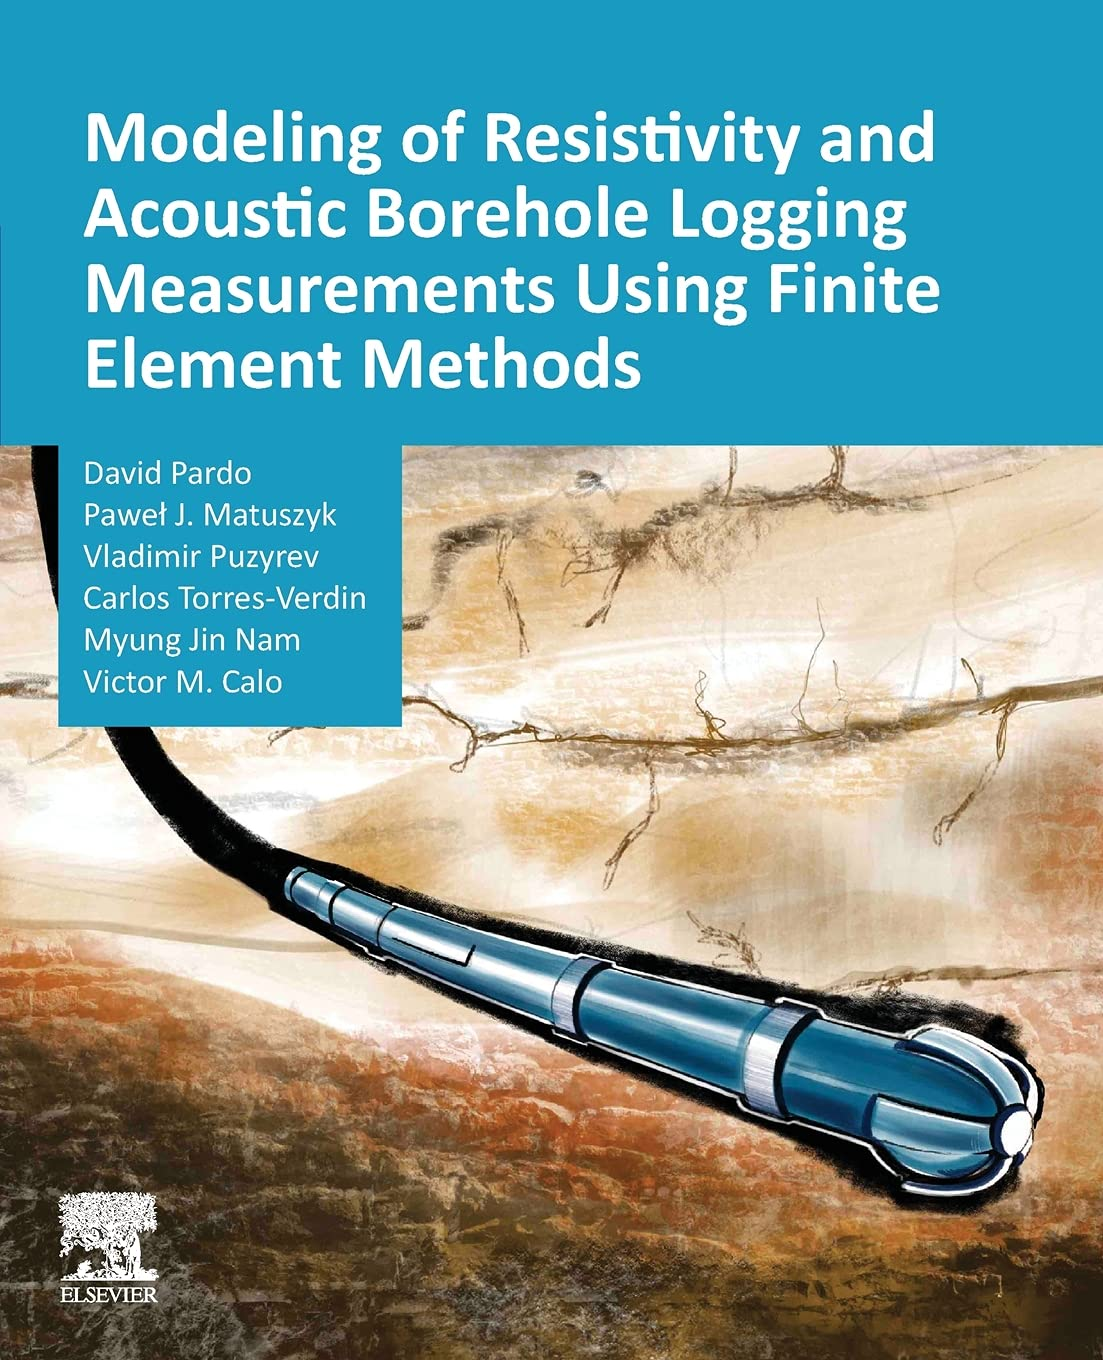
\includegraphics[width=0.8\textwidth]{Diapos/Intro/Figures/PardoBook.jpg} % Using width=\textwidth instead of scale
	\caption{Published in 2021} % Optional caption for the figure
	\label{fig:book} % Label for referencing the figure if needed
	\end{figure}
    \end{column}
    \begin{column}{0.48\textwidth}
      \begin{block}{Numerical Methods}
        \begin{itemize}
          \setlength\itemsep{2.4em} % Adjust the space between items
          \item Finite Element method
          \item Finite Difference method
          \item Finite Volumes method
          \item Integral methods
          \item Semi-analytical methods
        \end{itemize}
      \end{block}
    \end{column}
  \end{columns}
\end{frame}